\documentclass[a4paper,12pt]{article}

\usepackage[french]{babel}
\usepackage[utf8]{inputenc}
\usepackage[T1]{fontenc}
\usepackage{geometry}
\usepackage{graphicx}
\usepackage{float}
\usepackage{fancyhdr}
\usepackage{titlesec}
\usepackage[pdftex,pdfborder={0 0 0}]{hyperref}
\usepackage{mathpazo} % Utilisation de la police Palatino

% Mise en page
\geometry{margin=2.5cm}

% Configuration de fancyhdr pour les entêtes et pieds de page
\pagestyle{fancy}
\fancyhf{} % Efface tous les en-têtes et pieds de page existants

% En-tête
\fancyhead[L]{
\includegraphics[width=2cm]{../assets/img/logo_ensibs.png}}
\fancyhead[C]{\textbf{RSA power analysis attack with ChipWhisperer}}
\fancyhead[R]{\thepage}

% Pied de page
\fancyfoot[C]{}

% Personnalisation des sections
\titleformat{\section}{\normalfont\Large\bfseries}{\thesection}{1em}{}
\titleformat{\subsection}{\normalfont\large\bfseries}{\thesubsection}{1em}{}
\titleformat{\subsubsection}{\normalfont\normalsize\bfseries}{\thesubsubsection}{1em}{}


\begin{document}

% Page de garde
\begin{titlepage}
  \vspace*{-2cm}
  \hspace*{-2cm}
\includegraphics[scale=0.6]{../assets/img/logo_ensibs.png}
  \vspace*{-2cm}
  \hspace*{7cm}
\includegraphics[scale=0.6]{../assets/img/logo_ubs.png}\par
  \vspace{4cm}
  \centering
  {\scshape\LARGE \textbf{ENSIBS} \par}

  \vspace{1cm}
  {\scshape\Large PRJ 1401 \par}
  \vspace{1cm}
  \rule{\linewidth}{0.4mm}\par % Largeur de \linewidth et épaisseur de 0.7mm
  \vspace{1cm}
  {\huge\bfseries RSA power analysis attack with ChipWhisperer \par}
  \vspace{1cm}
  \rule{\linewidth}{0.4mm}\par % Largeur de \linewidth et épaisseur de 0.7mm
  \par
  \vspace{1cm}
  {\Large\itshape Cizdziel Matthieu, Richard Etienne, Moguedet Mathis\par}
  \vspace{1cm}
  {\Large\itshape PEI-2\par}
  \vspace{3cm}
  \par
  \vfill
  {\large \today\par}
\end{titlepage}

\newpage

% Table des matières
\tableofcontents
\newpage

% \begin{figure}[H]
%   \centering
%   \includegraphics[scale=1]{nom_du_fichier.png}
%   \caption{nom du graphique}
% \end{figure}

% Contenu du TP
\section{ChipWhisperer}
\subsection{ChipWhisperer's purpose}
ChipWhisperer is used to make power analysis attacks easy by making a confined environment that we can analyze. It also provides a lot of crypto-firmware that we can attack with some side channel attack's tutorials.
\subsection{ChipWhisperer's components }

\noindent ChipWhisperer is made of 2 main components :
\begin{itemize}
\item{a capture board used to record the current consumption and make the interface between the computer and the crypto-processor}
\item{a target board used to plug a target chip onto.The target board is useful to quickly switch from a target chip to another one} 
\end{itemize}

The target chip is the place where the firmware we want to analyze is running. This chip is only running our firmware so we don't have electrical noise on the analysis. The capture board is used to send the request to the target device and receive the output of the firmware, this board also record the current consumption of the target device. By slicing the work of a computer with two boards, the ChipWhisperer tool allow us to run our firmware in a confined space.

\pagebreak
\section{First attack on RSA}
For our first side channel attack on RSA we used an open source firmware and notebook found on github.
This firmware use the square and multiply algorithm so the attack was based on it.
Theses opensource files helped us to understand the using of simpleserial, a Chipwhisperer's library.
Finally we got the following output from the capture-board.

\begin{figure}[H]
  \centering
  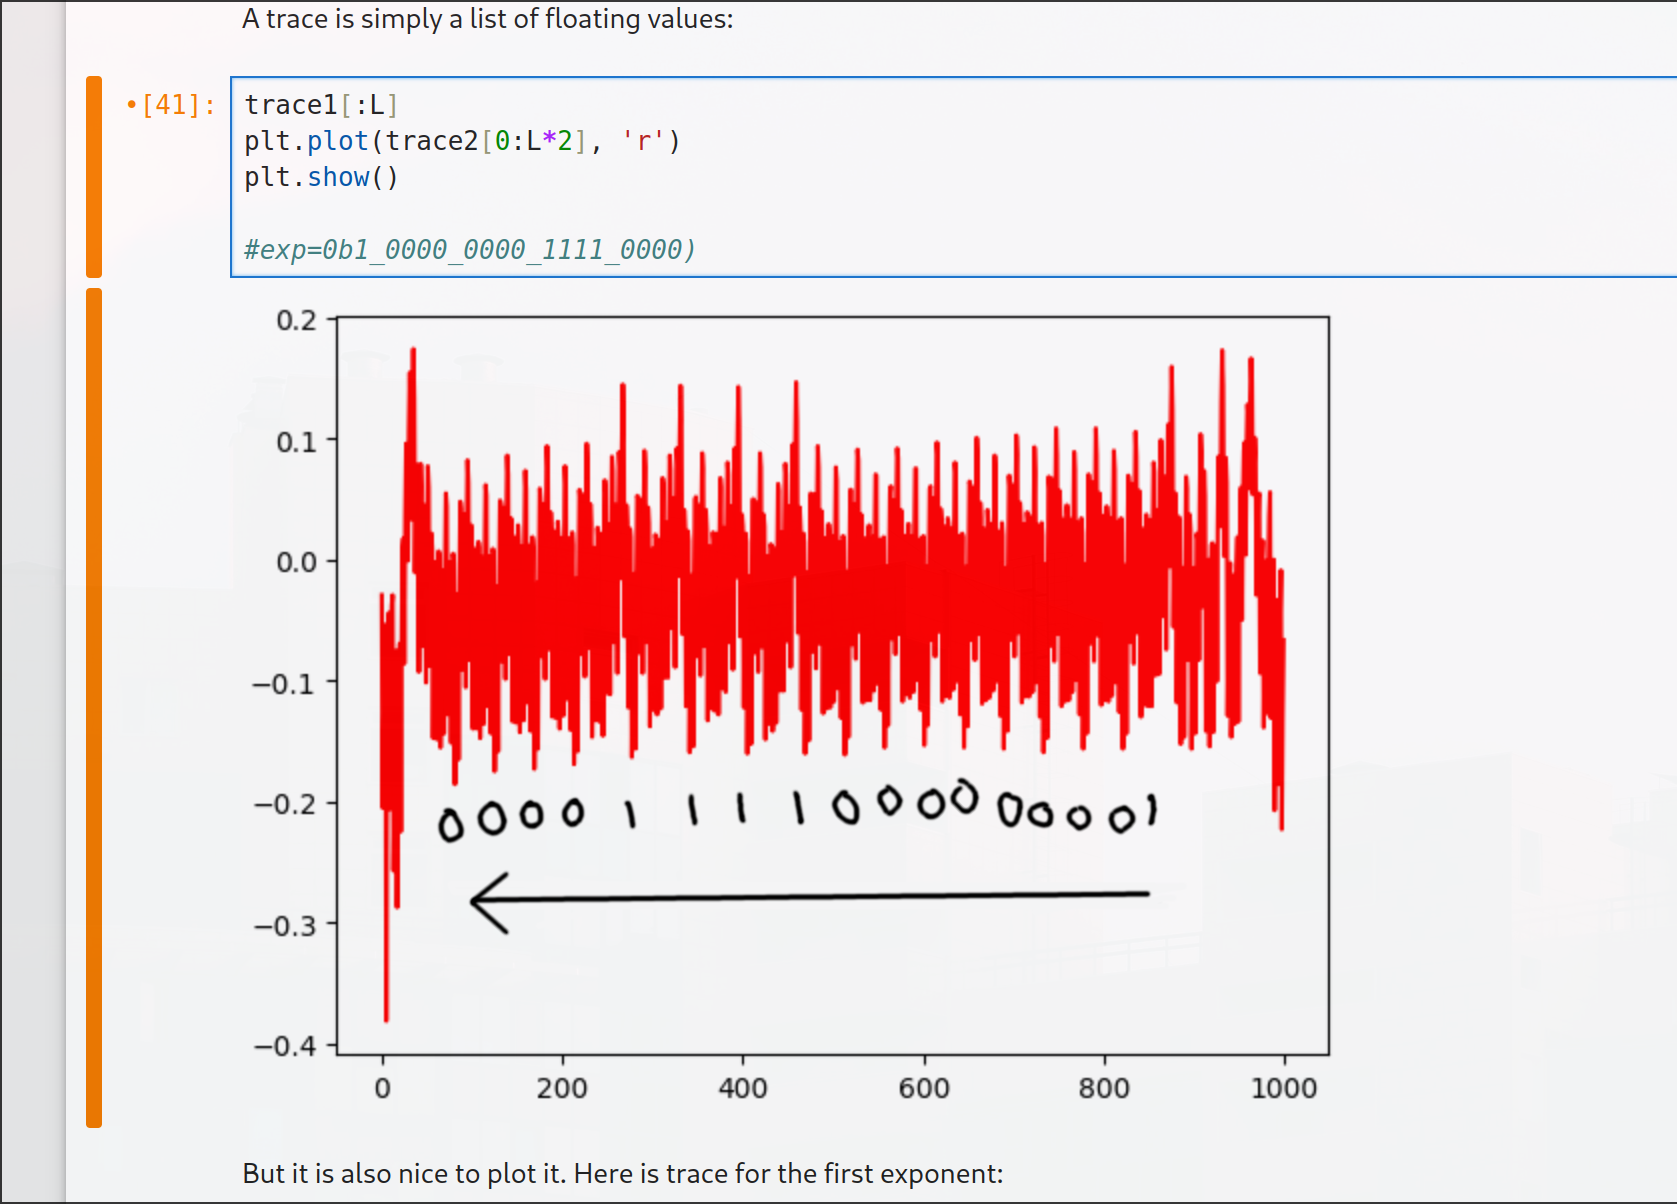
\includegraphics[width=0.7\textwidth]{../assets/img/first_attack.png}
  \caption{Currant consumption of the target}
\end{figure}

As we can see for every bit of the private key we can retrieve to correct value.


\section{Building our own Firmware}
\subsection{Communication between the computer and the ChipWhisperer}
To send the information from the computer to the ChipWhisperer, we use the "simpleserial.h" librairy.

% Votre discussion ici...
\section{Contexte du projet}
\subsection{Introduction}
En terme de sécurité informatique les méthodes de chiffrement sont très importantes notamment dans le domaine des télécommunication. La cryptographie est donc une notion très importante dans la cybersécurité actuelle. Les 3 principes de la cryptographie sont la confidentialité, l'authenticité et l'intégrité.
La confidentialité assure que le contenu d'un message chiffré ne peut être lu que par son destinataire.
L'authenticité assure l'origine du message, c'est à dire l'identité du messager.
Enfin l'intégrité assure la non-modification d'un message.
Dans notre cas nous mettrons en oeuvre des moyens pour s'attaquer à la confidentialité d'un protocole cryptographique. 
Ainsi nous allons vous présenter un algorithme connu pour sa robustesse et utilisé dans le monde entier, le protocole RSA.
\newpage
\subsection{Généralités sur le RSA}
Nous ne pouvons pas commencer la présentation du projet sans présenter le protocole RSA.
Le protocole RSA utilise une clé publique pour chiffrer le message et une clé privé pour le déchiffrer. Les clés publique et privé n'étant pas les mêmes, on parle de chiffrement asymétrique.
La robustesse du RSA repose dans la difficulté de factoriser un produit de deux grands nombres premiers.
Sans rentrer dans le détail de sa robustesse nous allons vous expliquer son fonctionnement:


\textbf{Génération des clés}
Soit $p$ et $q$ deux nombres premiers distincts. On pose alors $n=pq$ et $\phi(n)=(p-1)(q-1)$.
On choisit ensuite un nombre $e$ premier avec $\phi(n)$ et strictement inférieur à $\phi(n)$
On peut enfin calculer $d$ l'inverse modulaire de $e$ modulo $\phi(n)$.
Ainsi le couple (n,e) constitue la clé publique et $d$ la clé privée.


\textbf{Chiffrement}
Soit un message représenté par un entier naturel M strictement inférieur à n et C le message chiffré.
Nous avons la relation suivante:
\[
C \equiv M^e \pmod{n}
\]

\section{Conclusion}
% Votre conclusion ici...

\end{document}
